\documentclass[DM,lsstdraft,toc]{lsstdoc}

\usepackage[english]{babel}
\usepackage[utf8x]{inputenc}
\usepackage{amsmath}
\usepackage{graphicx}
\usepackage{longtable}
\usepackage{hyperref}
\usepackage{comment}
\usepackage{natbib}

\excludecomment{changelog}
\excludecomment{todo}
\excludecomment{openissues}

% Local commands go here
\newcommand{\G}[1]{{\color{green} #1}}
\newcommand{\B}[1]{{\color{blue} #1}}
\newcommand{\R}[1]{{\color{red} #1}}

%% Journal abbreviations
\bibliographystyle{aasjournal}

\title[LSST Science Platform]{LSST Science Platform Vision Document}

\author{
M.~Juri\'c,
D.R.~Ciardi,
and
G.P.~Dubois-Felsmann
}

\setDocRef{LDM-nnn}
\date{\today}
\setDocRevision{1.0}
\setDocStatus{draft}

\setDocAbstract{%

This document defines the high-level vision for the {\bf LSST Science
Platform (LSP)}, a set of web applications and services through which the
the scientific community will to access, visualize, interact with,
and analyze LSST data holdings.
\\

It is meant to inform the development of requirements, product specifications,
prioritization, and plans for the elements of the DM system that together 
comprise
the LSP.

}

% Change history defined here. Will be inserted into
% correct place with \maketitle
% OLDEST FIRST: VERSION, DATE, DESCRIPTION, OWNER NAME
\setDocChangeRecord{%
\addtohist{1}{2017-03-15}{Initial high-level description of the concept}{Mario 
Juric}
\addtohist{1}{2017-04-15}{Filling in view developed from Science Platform 
Vision document}{David Ciardi}
%\addtohist{2}{yyyy-mm-dd}{Future changes}{Future person}
}

\begin{document}

% Create the title page
% Table of contents will be added automatically if "toc" class option
% is used.
\maketitle

\section{Introduction}
The purpose of this document is to outline and document the vision that has been 
developed for the LSST Science Platform, and how we envision enabling the 
scientific user community being able to access the data, visualize the data, and 
interact with the data.   This is not a design document, but rather a document 
to aid in the definition of the requirements (both functional and 
non-functional) and in the definition of the design and interfaces.

The LSST is a facility whose primary mission is to acquire, process, and make 
available the data collected by its telescope and camera, as well as enable 
``next-to -the-data'' creation of added-value (Level 3) data products 
\cite{SRD}.  This document describes the vision for the services to be put into 
place to fulfill the `` {\em making available}'' and the ``{\em Level 3} 
creation`` aspects of LSST's mission. The aim of this document is to present a 
high-level description of the data access and analysis services provided at the 
LSST Data Access Centers.

\subsection{Goals and Philosphy of the Science Platform}

The LSST Science Platform is the entry point of the community to access the LSST 
data; the primary purpose of the Platorm is 1) to enable access to the LSST data 
products, 2) enable visualization and exploration of the LSST data, and 3) 
provide an interface to added-value processing and analysis close to the data.  
The customers of the Platform are the LSST Data Rights Scientists, the LSST 
Science Collaborations, and the LSST Project members.  

There is a continuum of users, user experiences, and user expertise with regards 
to the LSST project, data, and services.  As a result, the Platform needs to be 
simple enough to enage the general users and flexible enough to meet the needs 
of the more experienced users. Further, there is an expectation that user 
experiences and expertise will grow and adapt with time. 

In order to support this range of users, the Platform needs to provide both a 
structured environment with the LSST contextual information embedded in the 
system enabling users to learn about the data while at the same time providing a 
flexible environment for experienced users to perform more complex analyses.  
Toward achieving these goals, there are two connected aspects to the Platform: 
the Portal- aspect and the Notebook-aspect.  Each of these aspects is intended 
to enable a seamless flow across functionality and user experiences (see Figure~
\ref{fig:continuumSP}).
\begin{figure}
\centering
\scalebox{0.2}{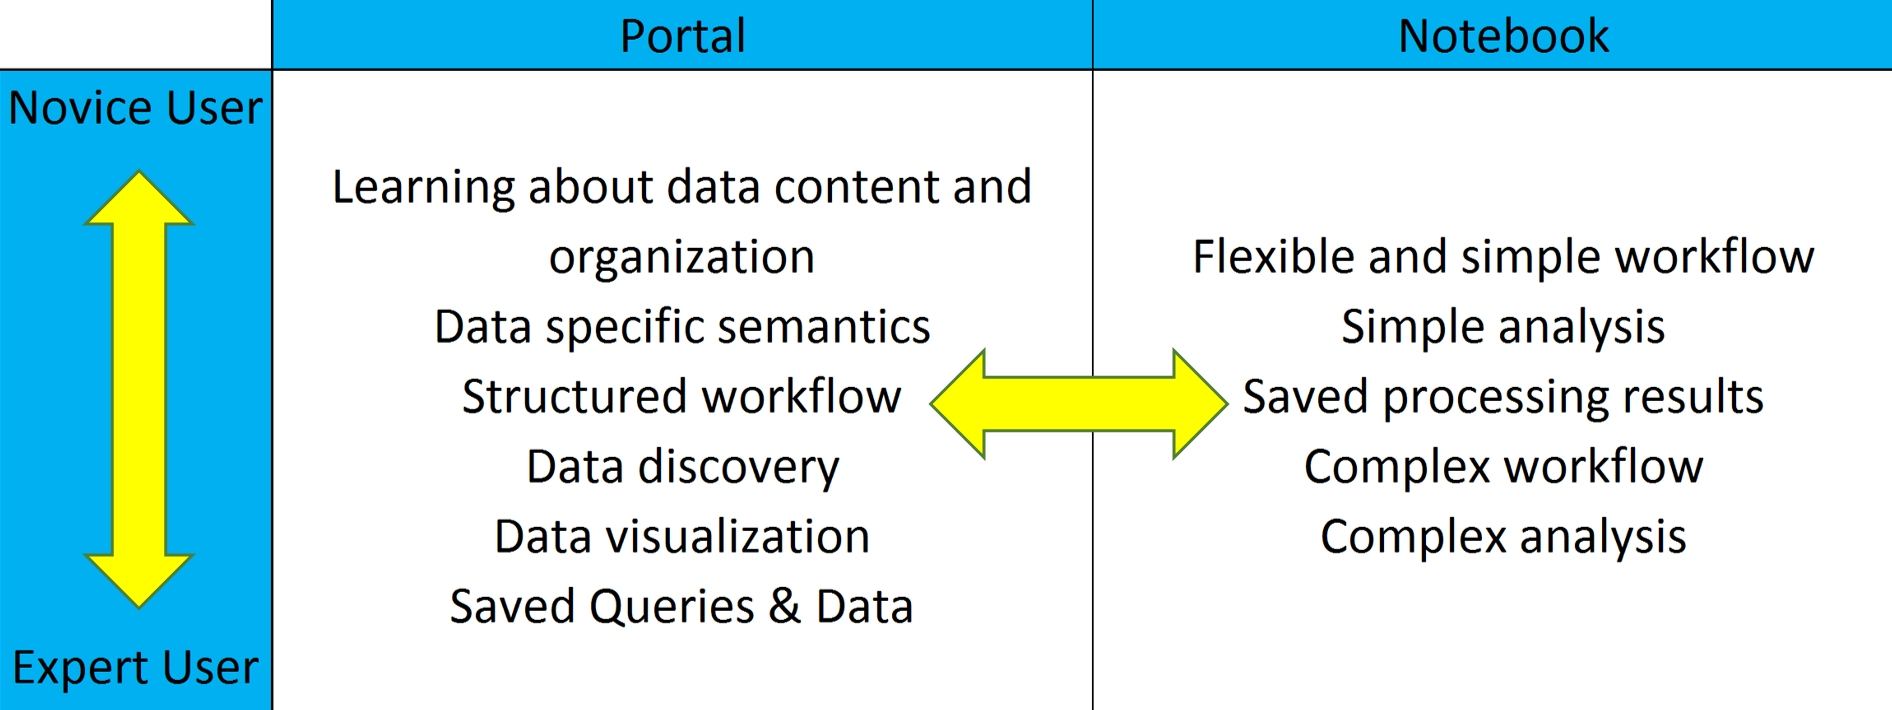
\includegraphics{images/fig-continuum_of_use}}
\caption{
A conceptual diagram describing the continuum of uses and user experiences 
expected to be supported by the LSST Science Platform). 
\label{fig:continuumSP}}
\end{figure}

The primary goals of the Platform are to provide a portal with a structured 
workflow that utilizes the LSST semantic contextual information about the data 
to enable users to explore and understand the data while at the same time 
providing a flexible computational environment that has access to the Data 
Products and the computational infrastructure.  Further, the Platform needs to 
enable the users to move between the portal and the flexible environments as 
their needs dictate.  By enabling connectivity between the structure environment 
of the Portal-aspect and the flexible environment of the Notebook-aspect, we can 
enable and encourage creativity in the use of the LSST data 
(Figure~\ref{fig:aspectsSP}).
\begin{figure}
\centering
\scalebox{0.15}{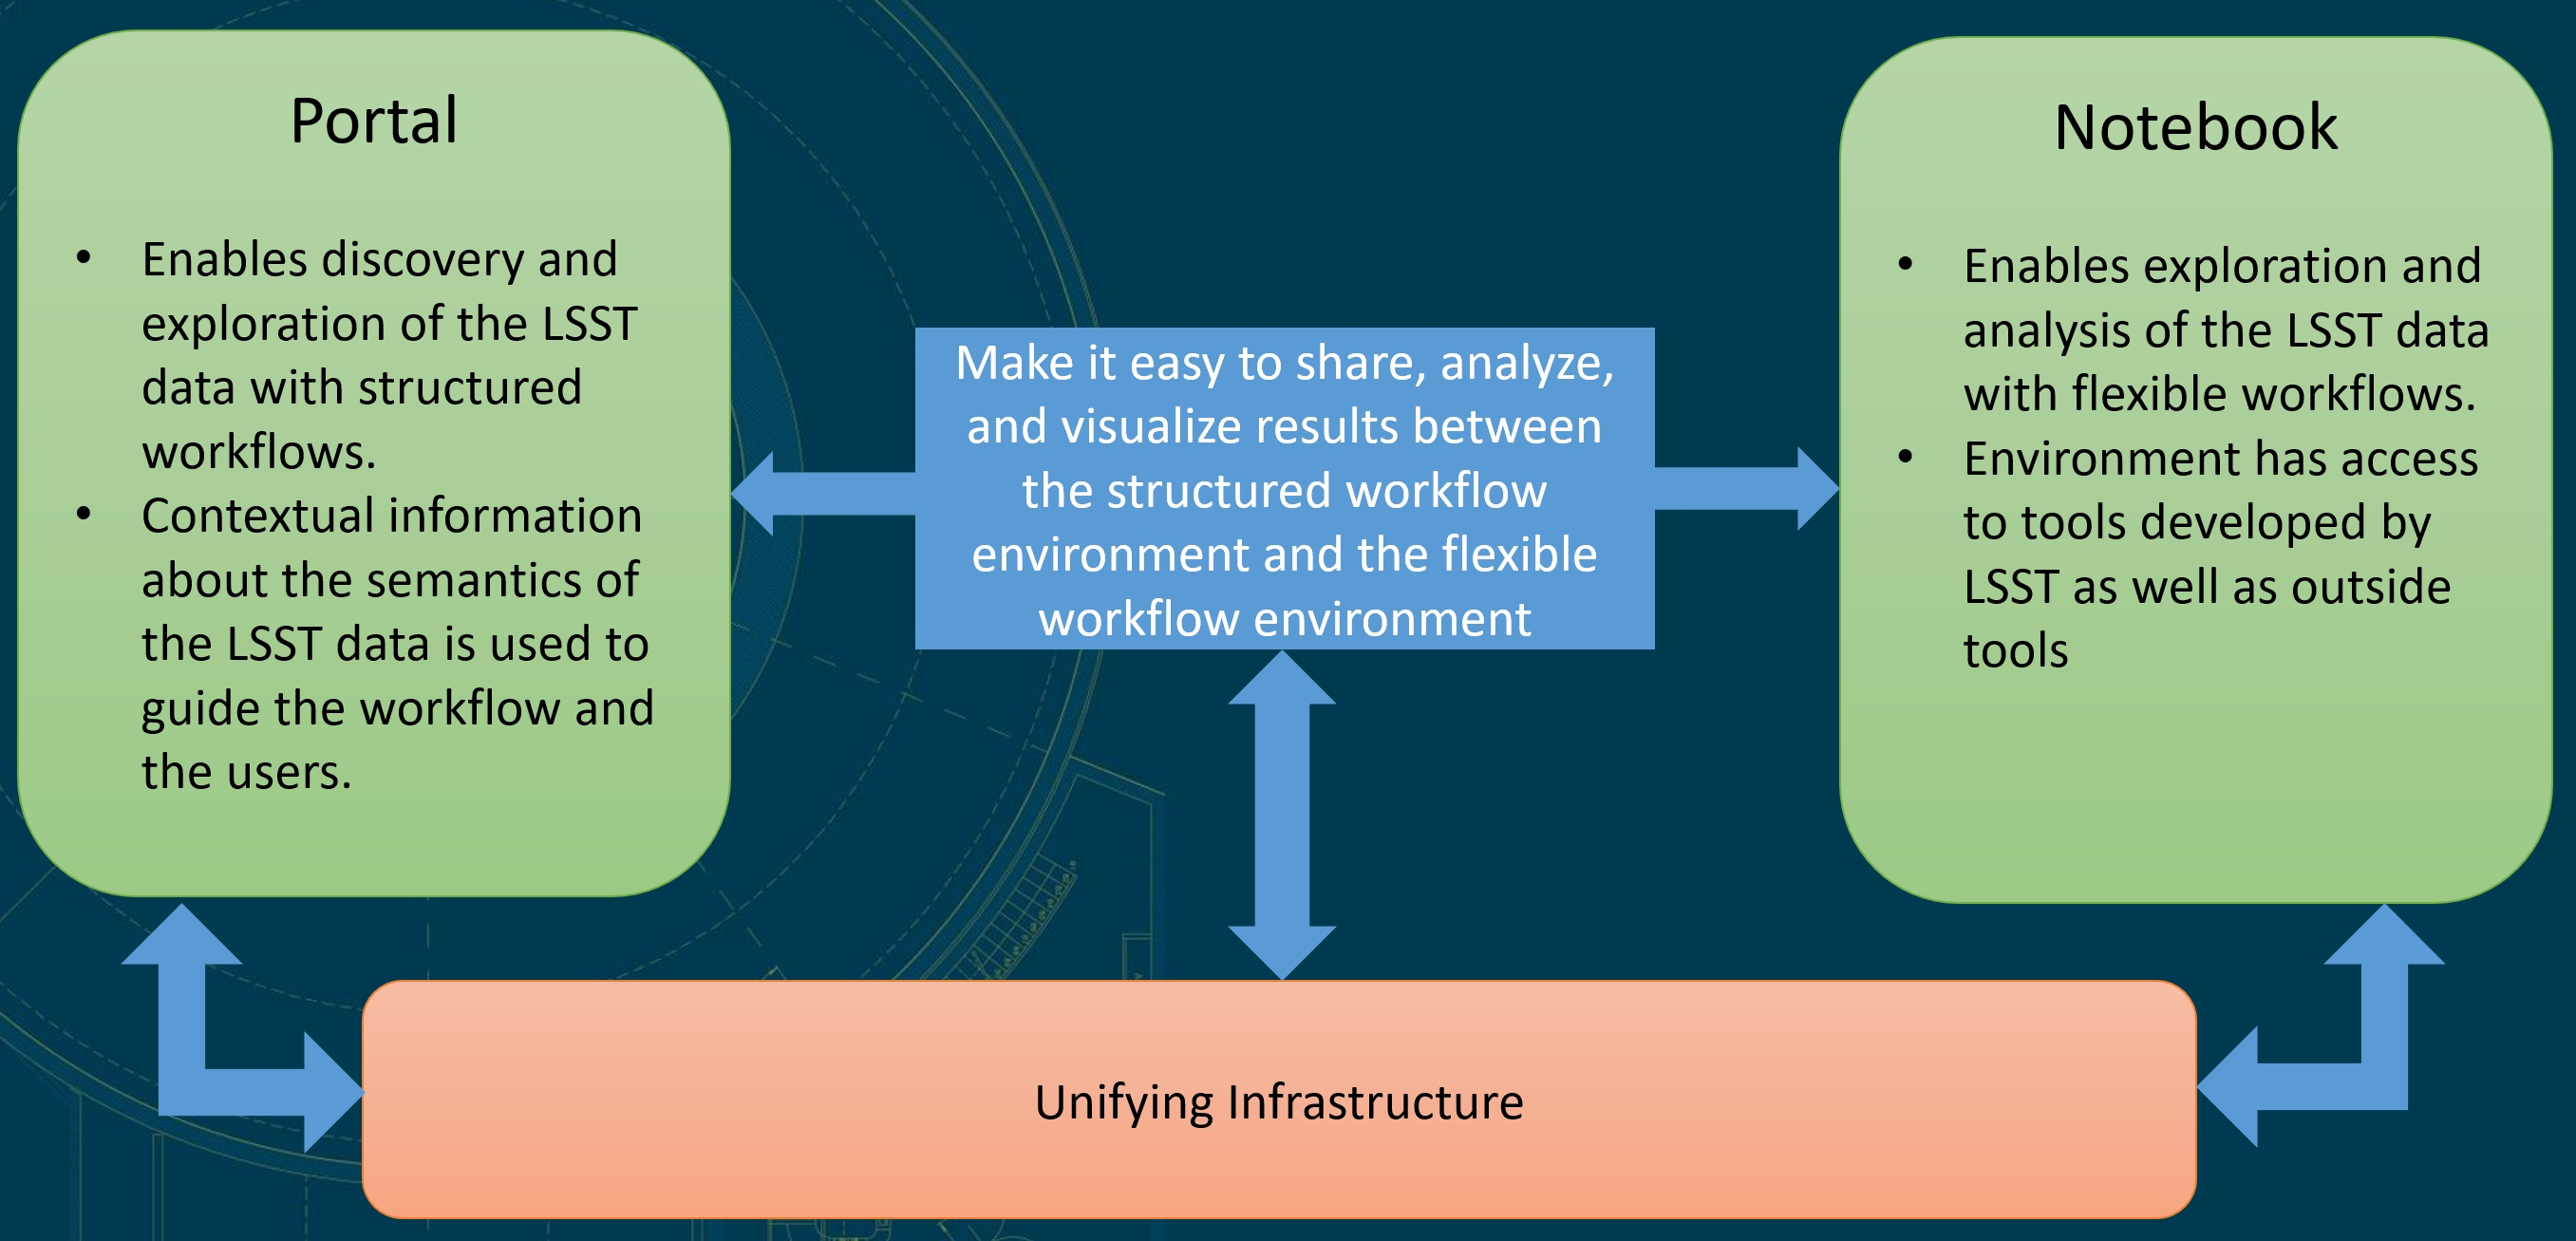
\includegraphics{images/fig-aspects}}
\caption{
A conceptual diagram showing the connectivity of the Portal and Notebook aspects 
of the Platform and the functional goals that the two aspects provide. 
\label{fig:aspectsSP}}
\end{figure}

The breadth of science possible with the LSST data is almost as endless and 
varied as the Universe itself and there is no way we can implement (or 
anticipate) all the specific needs and wants of the scientific community.  By 
making the Science Platform an environment in which the users can work and 
explore, we will enable the community to be imaginative in how they utilize the 
LSST data.

\subsection{LSST Science Platform Overview}

We define the LSST Science Platform as a set of web applications and services 
made available to the scientific community to access, visualize, subset, and 
perform next-to-the-data analysis of the LSST data set.  The platform can be 
thought of as exposing three primary user-facing ``aspects'' -- the web Portal, 
the Notebook analysis environment, and a machine-accessible Web API interface -- 
and a number of infrastructure elements supporting its function.  
(Figure~\ref{fig:layeredLSP}). 
\begin{figure}
\centering
\scalebox{0.4}{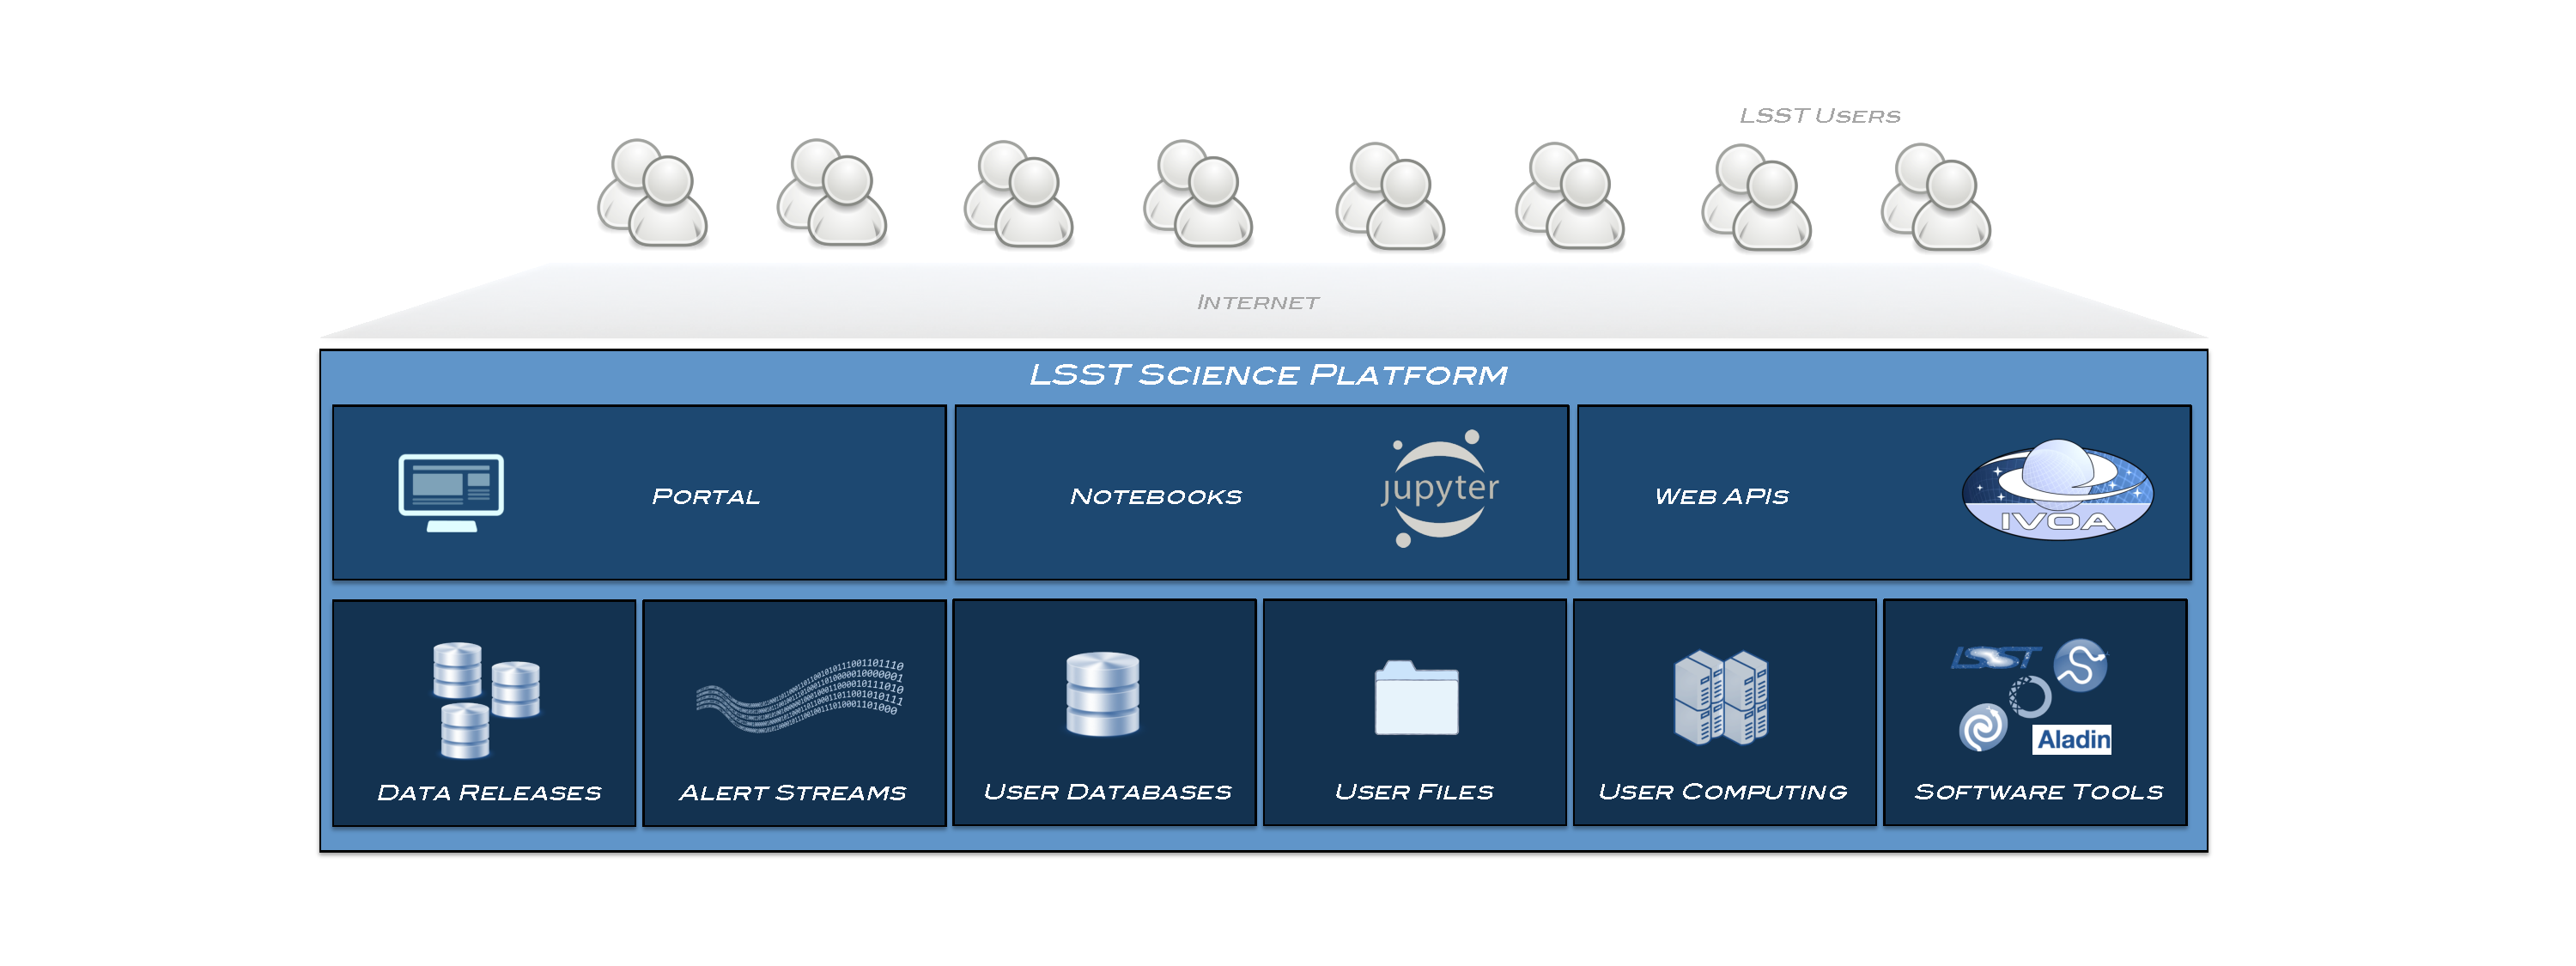
\includegraphics[trim={5cm 0.5cm 3cm 0.5cm},clip,page=1]
{images/fig-lsst-science-platform-extended}}
\caption{
A high-level, layered, view of the LSST Science Platform.  The LSST data will be 
exposed to the users through the Portal-aspect of the Platform, the Notebook- 
aspect interface, and machine-accessible Web APIs. 
\label{fig:layeredLSP}}
\end{figure}

Each aspect of the Platform will be connected with a unifying infrastructure 
that can be used to store and exchange data resulting from searches and analysis 
within each aspect of the Platform.  In particular, the aspects of the Platform 
rely upon the underlying DAX services and the NCSA provisioning services

The Portal-aspect will provide the essential data access and visualization 
services common to present day archives, while being connected to the 
infrastructure.  The Portal-aspect will provide the necessary contextual 
information for the users in order to help them explore the data and understand 
the connections between the various data products. 

The Notebook-aspect, based on the Jupyter family of technologies (e.g., 
JupyterHub and JupyterLab) will have access to the data saved by the users in 
the Portal-aspect, but will also have direct access to the data products and 
underlying infrastructure.  The Notebook-aspect will enable more sophisticated 
next-to-the-data analysis.  The results of the Notebook-aspect will also be 
available to the Portal-aspect for visualization and exploration.  

Each of these aspects and services will provide access to the underlying core 
LSST data sets -- the data releases and alert streams -- and be supported by 
the user Database, File Storage, Computing, and Software Tools components.  
Together, they will enable the users to access, sub-select, analyze, and perform 
added-value processing of all flavors of LSST Data Products.

The Portal and Notebook aspects of the Platform will be connected enabling a 
seamless workflow for the users to be able to move back and forth between these 
aspects as needs dictate.  As such, users are not confined to one aspect or the 
other.  The connections between the two aspects of the Science Platform are 
enabled by the common DAX architecture and computing infrastructure, the use of 
Javascript tools for visualization in both the Portal and the Notebook, and the 
rich data access and visualization APIs.  All of this enables a user to find or 
create data in one aspect and view or analyze that data in the other aspect.

As an example of how these connections can aid a user in exploring the LSST 
Data, data queries are shareable across the Portal and the Notebook which allows 
a user to build a query in the Portal user interface; the results can be 
verified by browsing it in the Portal, and then the results can be accessed from 
the Notebook for further analysis.  The reverse flow is also enabled; a user can 
code a complex SQL query in the Notebook and then browse the results in the 
Portal.  Additionally, the services will enable a user to capture a query 
formulated in the Portal as code reusable later as a Notebook-driven query, 
rather than just the data themselves, enabling pilot-run tests in the Portal 
followed by long-running more detailed analysis in the Notebook.  These 
Portal-Notebook connections can be made either through identity management (DAX 
knows the queries you have recently performed) or through simple UI actions 
(e.g., copy/paste of a query token between windows).

Finally, The LSST Science Platform is being designed to allow for collaborative 
work. Multiple users can share a Portal view or a Notebok enabling the system 
for collaborative use.  With LSST-aware visualizations developed for the Portal 
usable in the Notebook, the user experience is common across both aspects of the 
Platform, and the duplication of development effort by the community users is 
minimized.   The sharing capabilities of the platform will sharing of derived 
datasets within smaller groups, collaborations, or with the broader LSST 
community and extend to collaborative visualization and editing capabilities 
expected to become available within the Jupyter ecosystem.

\section{Enabling Remote Data Access and Analysis}

\subsection{Web Portal}
The Portal component is a web portal designed to provide the essential data 
access and visualization services through a simple-to-use website.  It will 
enable browsing and visualization of the available datasets in ways the users 
are accustomed to at archives such as IRSA, MAST, or the SDSS archive, with an 
enhanced level of interactivity in line with expectations for then-contemporary 
archive portals.  Through the Portal, the users will be able to view the LSST 
images, request subsets of data (via simple forms or SQL queries), store the 
results of such queries to their personal workspaces, construct commonly 
requested plots, and generally explore the LSST dataset in a way that allows 
them to identify and access (subsets of) data required by their science case.

\subsection{Jupyter Notebooks}
The Notebook environment, based on the Jupyter family of technologies (e.g., 
JupyterHub and JupyterLab), will be provided to allow for more sophisticated 
data selection, analysis, and creation of added value (Level 3) data products.  
The Notebook environment will come preinstalled with a library of commonly used 
and useful software Tools (such as AstroPy, LSST software stack, Anaconda 
Scientific Python Distribution, and others).  The users will be able to upload 
and install their own tools as well.

The Notebook user experience will be nearly identical to working with Jupyter 
notebooks locally, except that computation and analysis will occur at resources 
provided at the LSST Data Access Center.  This is an implementation of the 
“bringing computation to the data” paradigm: rather than imposing the burden of 
downloading, storing, and processing (large) subsets of LSST data at their home 
institutions, we will enable our users to bring their codes and perform their 
analysis at the LSST DAC.  We expect this will reduce the barrier to entry and 
shorten the path to science for the LSST science community.

\subsection{Web APIs}

\subsection{Computational Resources}
Queries, visualizations, and analysis performed through the Portal and Notebooks 
will be served by a shared computing cluster, file storage, and database 
resource (bottom row of Figure~\ref{fig:layeredLSP}).  At start of operations, 
this computing cluster will number 2,400 cores (approximately 18 TFLOPs), with 4 
PB of file and 3 PB of database storage (numbers for the U.S.  DAC). These will 
be shared by all users, the number of whom we’re estimating in the low 
thousands.

Not all users will be accessing the computing cluster concurrently; though 
difficult to predict with accuracy because of a lack of direct comparables, an 
estimate on order of a ~100 concurrent users is likely reasonable.  This would 
translate to typical allocations of ~20 cores per user, sufficient to enable 
preliminary end-user science analyses (working on catalogs, smaller number of 
images) and creation of some added-value (Level 3) data products. A good analogy 
is one of being given a server with a few TB of disk, few TB of database 
storage, that is co-located next to the LSST data, and with a chance to use tens 
to hundreds of cores for analysis (depending on system load).

For larger endeavors (e.g., pixel-level reprocessing of the entire LSST 
kdataset), the users will be steered towards resources beyond the LSST DACs 
(e.g., national supercomputing centers, university computing centers, or the 
public cloud).  Backend Science Platform services (including access to 
databases, images, and other files) will be exposed through machine-accessible 
web APIs serving community-accepted formats and protocols.  This will make it 
easy to initiate remote computations operating on LSST data.  Virtual 
Observatory interfaces will allow connection to other archives and enable the 
use of standard tools such as TOPCAT or Aladin. This will further lower the 
barrier to access to LSST data, shortening the path to science.


\section{Hosting Level 1 and 2: Database and Alert Filtering Services}

\subsection{Relational Databases}

\subsection{Alert Filtering Services}

\section{Enabling Level 3: User Databases, File storage, and Computing}

\subsection{Computing}

\subsection{File Storage}

\subsection{User Databases}

\end{document}
